\section{Arbeitslosigkeit}

Arbeitslosigkeit existiert dann, wenn Haushalte bereit sind, zum Marktlohn
Arbeit anzubieten, diese aber nicht von den Unternehmen nachgefragt werden.

Keine Arbeitslosigkeit herrscht dann, wenn Haushalte den Marktlohn als zu tief
empfinden und deshalb keine Arbeit anbieten (freiwillige Erwerbsunt�tigkeit).

\subsection{Typen der Arbeitslosigkeit \ho{Ho3 F12}}

Sockelarbeitslosigkeit: Anzahl der offenen Stellen ist gleich gross oder gr�sser als die
Anzahl der Arbeitslosen (strukturelle und friktionelle Arbeitslosigkeit).

Konjunkturelle Arbeitslosigkeit: Anzahl der Arbeitslosen ist gr�sser
als Anzahl der offenen Stellen.

\subsection{Kenngr�ssen des Arbeitsmarktes \ho{Ho3 F14}}

$$\textrm{Arbeitslosenquote} = \frac{\textrm{Arbeitslose}}{\textrm{Erwerbsbev�lkerung}} \cdot 100$$
$$\textrm{Erwerbsquote} = \frac{\textrm{Erwerbsbev�lkerung}}{\textrm{15- bis 64-J�hrige}} \cdot 100$$
$$\textrm{Erwerbst�tigenquote} = \frac{\textrm{Besch�ftigte}}{\textrm{15- bis 64-J�hrige}} \cdot 100$$

\subsection{Sockelarbeitslosigkeit}

Erkl�rungen f�r strukturelle Arbeitslosigkeit: Mindestl�hne, zentralisierte
Lohnverhandlungen, Regulierungen bez. Anstellungen und Entlassungen,
Ausgestaltung der ALV (Bezugsh�he), Regulierungen der Arbeitszeit

Erkl�rungen f�r friktionelle Arbeitslosigkeit: Ausgestaltung der ALV
(Bezugsdauer), Zeitspanne bis Finden einer neuen Stelle

\subsection{Konjunktur und Arbeitslosigkeit \ho{Ho4}}
\begin{multicols}{2}
	\subsubsection{Makro�konomisches Grundmodell}
		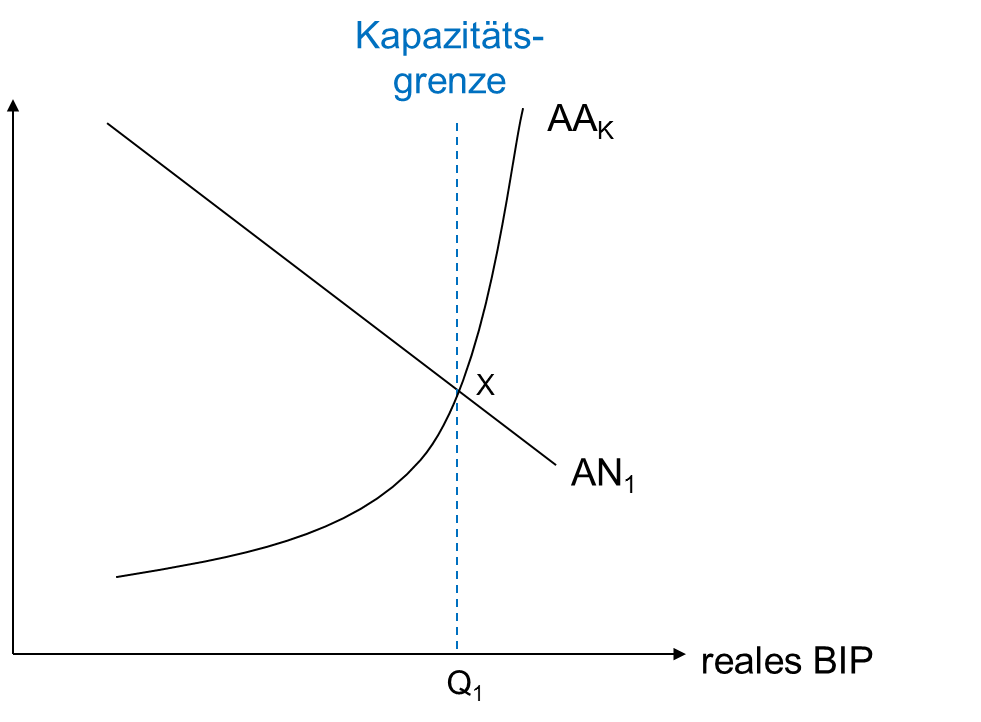
\includegraphics[width=9cm]{./bilder/h08f08.png}
	\subsubsection{Konjunkturelle Arbeitslosigkeit}
	  Entsteht durch einen Nachfrageschock und besteht nur kurzfristig.
			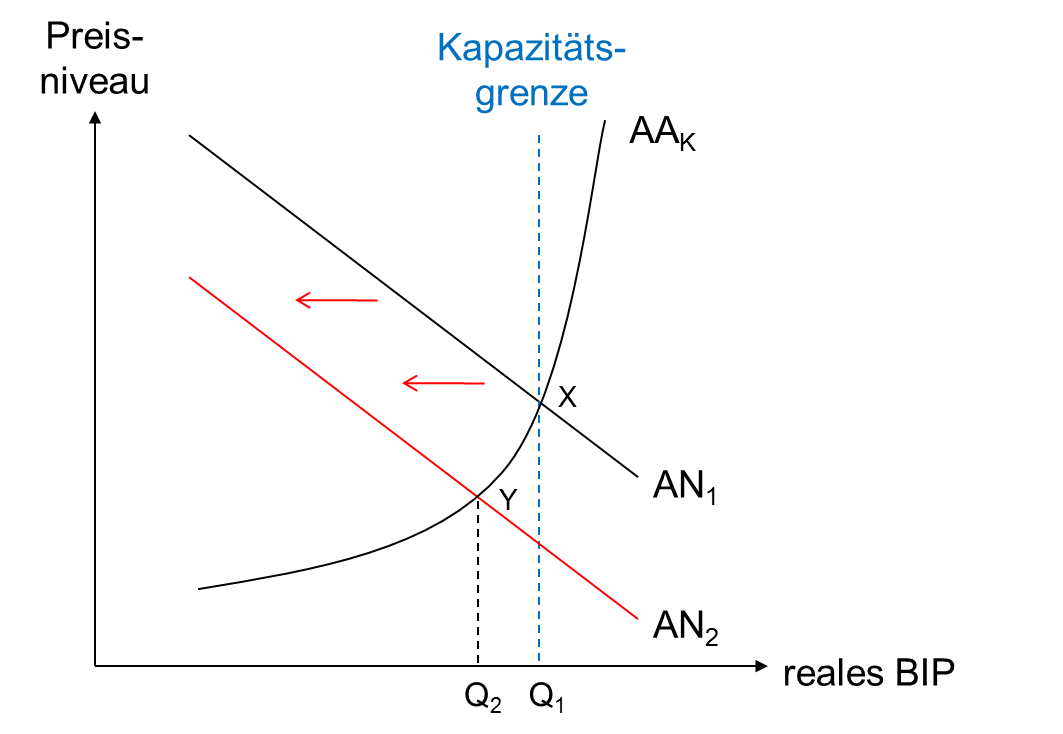
\includegraphics[width=9cm]{./bilder/h08f09.png} 
\end{multicols}

\subsubsection{Konjunkturpolitik \ho{Ho4 F8}}

Drei M�glichkeiten:

1. Nichts tun: Anpassung ohne aktive Konjunkturpolitik

2. Aktive "keynesianische" Konjunkturpolitik

3. St�rkung der automatischen Stabilisatoren

In der Schweiz wird vor allem auf automatische Stabilisatoren gesetzt:
Schuldenbremse, Arbeitslosenversicherung, Steuersystem.
